%%%%%%%%%%%%%%%%%%%%%%%%%%%%%%%%%%%%%%%%%%%%%%%%%%%%%%%%%%%%%%%%%%%%%%%%%%%
%
% Plantilla para un artículo en LaTeX en español.
%
%%%%%%%%%%%%%%%%%%%%%%%%%%%%%%%%%%%%%%%%%%%%%%%%%%%%%%%%%%%%%%%%%%%%%%%%%%%

% Qué tipo de documento estamos por comenzar:
\documentclass[a4paper]{article}
% Esto es para que el LaTeX sepa que el texto está en español:
\usepackage[spanish]{babel}
\usepackage{listings}
\selectlanguage{spanish}

% Esto es para poder escribir acentos directamente:
\usepackage[utf8]{inputenc}
\usepackage[T1]{fontenc}
\usepackage{bm}

\usepackage[usenames,dvipsnames]{color}    
\lstset{ 
  language=R,                     % the language of the code
  basicstyle=\ttfamily, % the size of the fonts that are used for the code
  numbers=left,                   % where to put the line-numbers
  numberstyle=\ttfamily\color{Blue},  % the style that is used for the line-numbers
  stepnumber=1,                   % the step between two line-numbers. If it is 1, each line
                                  % will be numbered
  numbersep=5pt,                  % how far the line-numbers are from the code
  %backgroundcolor=\color{white},  % choose the background color. You must add \usepackage{color}
  showspaces=false,               % show spaces adding particular underscores
  showstringspaces=false,         % underline spaces within strings
  showtabs=false,                 % show tabs within strings adding particular underscores
  %frame=single,                   % adds a frame around the code
  %rulecolor=\color{black},        % if not set, the frame-color may be changed on line-breaks within not-black text (e.g. commens (green here))
  tabsize=2,                      % sets default tabsize to 2 spaces
  captionpos=b,                   % sets the caption-position to bottom
  breaklines=true,                % sets automatic line breaking
  breakatwhitespace=false,        % sets if automatic breaks should only happen at whitespace
  %keywordstyle=\color{RoyalBlue},      % keyword style
  commentstyle=\color{ForestGreen},   % comment style
  %stringstyle=\color{Green}      % string literal style
} 

%% Asigna un tamaño a la hoja y los márgenes
\usepackage[a4paper,top=3cm,bottom=2cm,left=3cm,right=3cm,marginparwidth=1.75cm]{geometry}

%% Paquetes de la AMS
\usepackage{amsmath, amsthm, amsfonts}
%% Para añadir archivos con extensión pdf, jpg, png or tif
\usepackage{graphicx}
\usepackage[colorinlistoftodos]{todonotes}
\usepackage[colorlinks=true, allcolors=blue]{hyperref}

%% Primero escribimos el título
\title{Modelado estadístico de datos: Práctica 1 Feb 2021 }
\author{Jorge Pablo Ávila Gómez \date{} }

%% Después del "preámbulo", podemos empezar el documento
\setlength{\marginparwidth}{2cm}
\begin{document}
\renewcommand{\tablename}{Tabla} 
%% Hay que decirle que incluya el título en el documento
\maketitle

%% Aquí podemos añadir un resumen del trabajo (o del artículo en su caso) 
% \begin{abstract}
% Esta es una plantilla simple para crear un articulo \LaTeX en español, con algunos comandos que se usarán % frecuentemente para hacer tareas de la licenciatura en Física.
% \end{abstract}

%% Iniciamos "secciones" que servirán como subtítulos

\section{Ejercicio 1}
\textbf{Enunciado:}\par
Se ha realizado un estudio para ver si influye el tipo de tratamiento a la hora de evitar el dolor de cabeza en estudiantes en periodo de exámenes. Para ello 14 estudiantes han recibido el tratamiento $A$ y 20 el tratamiento $B$. De cada estudiante se ha registrado al final del periodo de exámenes su dolor de cabeza en una escala cuantitativa, de forma que a más valor mayor dolor. Los datos experimentales se encuentran en el fichero $dolor\_tratamiento\_2.txt$ ¿Hay diferencias estadísticamente significativas entre los dos tratamientos a la hora de evitar el dolor? \par
\textbf{Solución:}\par
El primer paso es entender el tipo de variables con las que estamos tratando. Vemos que existen dos tipos de tratamientos, $A$ y $B$, indicando que la variable explicativa es dicotómica. Por otro lado, vemos que la variable respuesta, dolor de cabeza, se ha medido en una escala cuantitativa, por tanto tenemos que es una variable continua. Nos encontramos por tanto ante un esquema $C \leftarrow D$. \par
El enunciado nos pregunta si hay diferencias estadísticamente significativas entre los dos tratamientos. Para contestar a esta pregunta vamos a plantear un contraste de hipótesis.
En el esquema $C \leftarrow D$ se suele utilizar el test $t$ de Student para el contraste de hipótesis. Pero, para poder aplicar este test hay que comprobar que las distribuciones de los dos tratamientos son normales. Para ello se usa el test de Shapiro a partir del siguiente código en \verb|R|:
\begin{lstlisting}[language=R]
data = read.table('dolor_tratamiento_2.txt', header = T)
attach(data)

ind1=which(exp==1) ## Tratamiento A
ind2=which(exp==2) ## Tratamiento B

shapiro.test(rta[ind1])
shapiro.test(rta[ind2])
\end{lstlisting}
Se obtiene para el tratamiento A un p-valor = 0.022 y para el tratamiento B un p-valor = 0.038. Los dos valores son menores que 0.05 por tanto, se rechaza la hipótesis nula. En el caso del test de Shapiro la hipótesis nula es que la distribución es normal, como la hemos rechazado para los dos tratamiento nos encontramos ante la situación de que ninguna de las dos distribuciones son normales. Por tanto no podemos aplicar el test $t$ de Student. \par
Como alternativa, vamos a utilizar el test $U$ de Mann-Whitney. Este test está enmarcado en el esquema $O \leftarrow D$, pero también se puede usar en el esquema $C \leftarrow D$ cuando no se cumple la asunción de normalidad.\par
Se propone el siguiente contraste de hipótesis, donde la hipótesis nula indicaría que no hay diferencia entre las funciones de distribución de los tratamientos, y la hipótesis alternativa que si las hay.
\[ H_0 : F_1 = F_2   \]
\[ H_1 : F_1 \ne F_2    \]
El test $U$ de Mann-Whitney se calcula con el siguiente código en \verb|R|:
\begin{lstlisting}[language=R]
wilcox.test(rta[ind1],rta[ind2], correct = FALSE)
\end{lstlisting}
Se obtiene un p-valor de 0.3927 > 0.05. Por tanto no hay evidencia suficiente para rechazar la hipótesis nula. Se consideran iguales las funciones de distribución y por tanto, se concluye que no hay diferencias significativas entre los dos tratamientos. 

\section{Ejercicio 2}

\textbf{Enunciado:}\par
En el modelo de regresión lineal, se define la matriz C (matriz de ``ortogonalización``) como la matriz dada por $\mathbf{C} = (\mathbf{X}^T\mathbf{X})^{-1}\mathbf{X}^T$, entonces se verifica que $\mathbf{C}\mathbf{C}^T = \mathbf{I}$. Verdadero o Falso.\par
\textbf{Solución:}\par
b) Falso \par

\[ \mathbf{C} = (\mathbf{X}^T\mathbf{X})^{-1}\mathbf{X}^T   \]
\[ \mathbf{C}\mathbf{C}^T = [(\mathbf{X}^T\mathbf{X})^{-1}\mathbf{X}^T][(\mathbf{X}^T\mathbf{X})^{-1}\mathbf{X}^T]^T =\]
Propiedades de la transpuesta: $(AB)^T = B^TA^T; (A^T)^T = A$
\[ = [(\mathbf{X}^T\mathbf{X})^{-1}\mathbf{X}^T][\mathbf{X}((\mathbf{X}^T\mathbf{X})^{-1})^T] = \]
Quitando corchetes:
\[ = (\mathbf{X}^T\mathbf{X})^{-1}\mathbf{X}^T\mathbf{X}((\mathbf{X}^T\mathbf{X})^{-1})^T = \]
Propiedad de la inversa: $A^{-1}A = I$
\[ = \mathbf{I}((\mathbf{X}^T\mathbf{X})^{-1})^T = \]
Propiedad de la inversa: $(A^{-1})^T = (A^T)^{-1}$
\[ = \mathbf{I}((\mathbf{X}^T\mathbf{X})^T)^{-1} = \]
Propiedad de la transpuesta: $(AB)^T = B^TA^T; (A^T)^T = A$
\[ = \mathbf{I}(\mathbf{X}^T\mathbf{X})^{-1} \]
El siguiente código en \verb|R| comprueba el resultado:
\begin{lstlisting}[language=R]
X = matrix(rnorm(40), ncol=4) # A random 10x4 matrix
C = solve(t(X) %*% X) %*% t(X) # C

tol = 1e-10
abs(C %*% t(C) - solve(t(X) %*% X)) <= tol # C C^T = (X^T X)^-1
\end{lstlisting}

\section{Ejercicio 3}

\textbf{Enunciado:}\par
En el modelo de regresión lineal, se define la matriz C (matriz de ``ortogonalización``) como la matriz dada por $\mathbf{C} = (\mathbf{X}^T\mathbf{X})^{-1}\mathbf{X}^T$, entonces se verifica que $\bm{\widehat{\beta}} = \bm{\beta} + \mathbf{C}\bm{\epsilon}$. Verdadero o Falso.\par
\textbf{Solución:}\par
a) Verdadero

Partiendo de la expresión:
\[ \bm{\widehat{\beta}} = \mathbf{C}\mathbf{y} = \]
Sustituimos $\mathbf{y} = \mathbf{X}\bm{\beta} + \bm{\epsilon}$ :
\[ = \mathbf{C}(\mathbf{X}\bm{\beta} + \bm{\epsilon}) = \]
\[ = \mathbf{C}\mathbf{X}\bm{\beta} + \mathbf{C}\bm{\epsilon} \]
Tenemos que demostrar que $\mathbf{C}\mathbf{X} = \mathbf{I}$
\[ \mathbf{C}\mathbf{X} = (\mathbf{X}^T\mathbf{X})^{-1}\mathbf{X}^T\mathbf{X} = \]
Propiedad de la inversa: $A^{-1}A = I$
\[ = \mathbf{I} \]
Por tanto tenemos:
\[ \bm{\widehat{\beta}} = \mathbf{I}\bm{\beta} + \mathbf{C}\bm{\epsilon} \]
Hemos demostrado la expresión.

\section{Ejercicio 4}

\textbf{Enunciado:}\par
Para los datos del fichero $c\_c\_1.txt$ alojado en el curso virtual, se pide, utilizando \verb|R|, lo siguiente:
\begin{itemize}
    \item Calcular los coeficientes de la recta de regresión de \verb|rta| en función de \verb|exp| y los $h_{ii}$ correspondientes.
    \item Crear una nueva variable \verb|expc| que sea el resultado de centrar \verb|exp| y calcular los coeficientes de la recta de regresión de \verb|rta| en función de \verb|expc| y los $h_{ii}$ correspondientes.
    \item Crear una nueva variable \verb|rtac| que sea el resultado de centrar \verb|rta| y calcular los coeficientes de la recta de regresión de \verb|rtac| en función de \verb|expc| y los $h_{ii}$ correspondientes.
    \item Interpretar los resultados obtenidos.
\end{itemize}
\textbf{Solución:}\par
Código utilizado:\par
\begin{lstlisting}[language=R]
rm(list=ls())
data = read.table('c_c_1.txt', header = T)
attach(data)
par(mfrow=c(1,1),pty="m")

# Punto 1
f1=lm(rta~exp)
f1
plot(exp,rta, xlim=c(-50, 100), ylim=c(-50, 100), pch=19, col="red")
abline(f1,col="red" )
# Punto 2
expc = exp - mean(exp) # Centrado
f2 =lm(rta~expc)
f2
points(expc,rta, pch=19, col="blue")
abline(f2, col="blue")
# Punto 3
rtac = rta - mean(rta) # Centrado
f3 =lm(rtac~expc)
f3
points(expc,rtac, pch=19, col="darkgreen")
abline(f3, col="darkgreen")

legend(-50,0,legend=c("rta~exp", "rta~expc", "rtac~expc"), col=c("red", "blue","darkgreen"),lty=1,)

# h_ii
hatvalues(f1)
hatvalues(f2)
hatvalues(f3)
# grafica h_ii
par(mfrow=c(1,3),pty='s')
plot(hatvalues(f1), pch=19, col="red")
plot(hatvalues(f2), pch=19, col="blue")
plot(hatvalues(f3), pch=19, col="darkgreen")

detach(data)
\end{lstlisting}
\begin{table}
    \centering
    \begin{tabular}{ c  c  c }
    Ajuste & Ordenada en y &  pendiente \\ \hline
    Punto 1 & 168.528   &    -1.176 \\
    Punto 2 & 80.750   &   -1.176 \\
    Punto 3 & -5.320e-15 & -1.176 \\
    \end{tabular}
    \caption{\label{tab:41}Coeficientes de las rectas de regresión.}
\end{table}
\begin{table}
    \centering
    \begin{tabular}{c c c}
    $h_{ii}$ punto 1 & $h_{ii}$ punto 2 &  $h_{ii}$ punto 3 \\ \hline
    0.09354067 & 0.09354067 & 0.09354067 \\
    0.11459330 & 0.11459330 & 0.11459330 \\
    0.14712919 & 0.14712919 & 0.14712919 \\
    0.26770335 &0.26770335 &0.26770335 \\
    0.37822967 &0.37822967 &0.37822967 \\
    0.23660287 &0.23660287 &0.23660287 \\
    0.11459330 &0.11459330 &0.11459330 \\
    0.14712919 &0.14712919 &0.14712919 \\
    0.11459330 &0.11459330 &0.11459330 \\
    0.11459330 &0.11459330 &0.11459330 \\
    0.14712919 &0.14712919 &0.14712919 \\
    0.12416268 & 0.12416268 &0.12416268\\
    \end{tabular}
    \caption{\label{tab:42}Coeficientes $h_{ii}$ para cada modelo.}
\end{table}
\begin{figure}
\centering
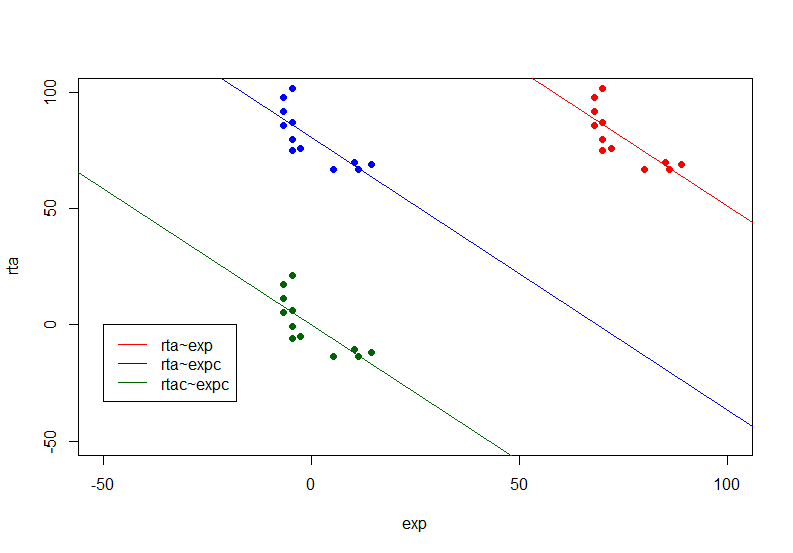
\includegraphics[width=0.8\textwidth]{4_1.png}
\caption{\label{fig:f41}Líneas de regresión.}
\end{figure}
\begin{figure}
\centering
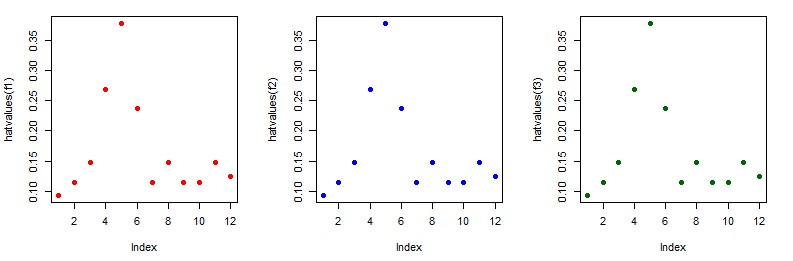
\includegraphics[width=1\textwidth]{4_2.jpg}
\caption{\label{fig:f42}Coeficientes $h_{ii}$.}
\end{figure}

Los coeficientes de cada ajuste se encuentran en la tabla~\ref{tab:41}, y en la figura~\ref{fig:f41} podemos ver los datos y las rectas de regresión. Los $h_{ii}$ correspondientes se encuentran en la tabla~\ref{tab:42} y la figura~\ref{fig:f42}. \par

El primer punto consiste en calcular los coeficientes de la recta. Estos se calculan por las fórmulas siguientes: 
\[ \hat{\beta}_1 = \frac{\sum_{i=1}^n(x_i - \bar{x})(y_i - \bar{y})}{\sum_{i=1}^n(x_{i} - \bar{x})^2} \]
\[ \hat{\beta}_0 = \bar{y} - \hat{\beta}_1\bar{x}\]
Donde $\hat{\beta}_1$ es la pendiente del ajuste del punto 1 y $\hat{\beta}_0$ la ordenada en el origen.\par
Al realizar el centrado en $exp$ obtenemos los nuevos valores de x y su media ($expc$): 
\[ x_{i\_expc} = x_{i} - \bar{x} \]
\[\bar{x}_{expc} = 0\]
Podemos calcular los coeficientes de la recta en el segundo ajuste, usando $expc$, sustituyendo los nuevos valores en la fórmula y simplificando: 
\[ \hat{\beta}_{1expc} = \frac{\sum_{i=1}^n(x_{i\_expc} - \bar{x}_{expc})(y_i - \bar{y})}{\sum_{i=1}^n(x_{i\_expc} - \bar{x}_{expc})^2} = \frac{\sum_{i=1}^n(x_{i} - \bar{x} - 0)(y_i - \bar{y})}{\sum_{i=1}^n(x_{i} - \bar{x} - 0)^2} \]
\[ \hat{\beta}_{0expc} = \bar{y} - \hat{\beta}_{1expc}\bar{x}_{expc} = \bar{y} - \hat{\beta}_{1expc} * 0 = \bar{y}\]
Vemos que el valor de la pendiente no cambia $\hat{\beta}_1 = \hat{\beta}_{1expc} $ y por otro lado el valor de la ordenada en el origen pasa a valer $\bar{y}$. \par
En el tercer punto centramos los valores de $rta$ que es la variable respuesta $y$, los valores de esta nueva variable serán:
\[ y_{i\_rtac} = y_{i} - \bar{y} \]
\[\bar{y}_{rtac} = 0\]
Calculamos los coeficientes de manera similar a como hemos hecho antes: 
\[ \hat{\beta}_{1expcrtac} = \frac{\sum_{i=1}^n(x_{i\_expc} - \bar{x}_{expc})(y_{i\_rtac} - \bar{y}_{rtac})}{\sum_{i=1}^n(x_{i\_expc} - \bar{x}_{expc})^2} = \frac{\sum_{i=1}^n(x_{i} - \bar{x} - 0)(y_i - \bar{y} - 0)}{\sum_{i=1}^n(x_{i} - \bar{x} - 0)^2} \]
\[ \hat{\beta}_{0expcrtac} = \bar{y}_{rtac} - \hat{\beta}_{1expc}\bar{x}_{expc} = 0 - \hat{\beta}_{1expc} * 0 = 0\]
Volvemos a comprobar que el valor de la pendiente no cambia $\hat{\beta}_1 = \hat{\beta}_{1expcrtac} $ y por otro lado el valor de la ordenada en el origen pasa a valer 0. \par
Estos resultados se corresponde a los encontrados experimentalmente. Se han obtenido tres líneas paralelas, tienen la misma pendiente, pero desplazadas en el plano x-y, porque tienen diferente ordenada en el origen (figura~\ref{fig:f41}). Podemos concluir que el centrado no cambia las distancias relativas entre los puntos, solo los desplaza en su conjunto, en consecuencia se mantiene la pendiente de la curva que mejor los ajusta. \par


Con respecto a los valores de $h_{ii}$ vemos que son iguales para los tres ajustes. Esto se puede explicar mediante la fórmula que calcula los valores $h_{ii}$ para una regresión lineal simple:
\[ h_i = \frac{1}{n} + \frac{(x_i - \bar{x})^2}{\sum_{i'=1}^n(x_{i'} - \bar{x})^2}       \]

Al sustituir los datos de $expc$ obtenemos: 
\[ h_{iexpc} = \frac{1}{n} + \frac{(x_{i\_expc} - \bar{x}_{expc})^2}{\sum_{i'=1}^n(x_{i'\_expc} - \bar{x}_{expc})^2} = \frac{1}{n} + \frac{(x_i - \bar{x} - 0)^2}{\sum_{i'=1}^n(x_{i'} - \bar{x} - 0)^2}        \]
Vemos que se obtienen los mismos valores de $h_{ii}$, explicando que experimentalmente $h_{i} = h_{iexpc}$. Por otro lado, vemos que en la fórmula no interviene la variable respuesta ($y$), por tanto el centrado de $rta$, en el último punto, no afecta a los valores de $h_{iexpcrtac}$, explicando que en el último ajuste se obtenga de nuevo los mismos valores para $h_{ii}$.

\section{Ejercicio 5}

\textbf{Enunciado:}\par
Para los datos del fichero $c\_c\_1.txt$ alojado en el curso virtual, se pide, utilizando \verb|R|, lo siguiente:
\begin{itemize}
    \item Crear una nueva variable \verb|exp10| que sea el resultado de multiplicar \verb|exp| por 10 y calcular los coeficientes de la recta de regresión de \verb|rta| en función de \verb|exp10| y los $h_{ii}$ correspondientes.
    \item Crear una nueva variable \verb|rta10| que sea el resultado de multiplicar \verb|rta| por 10 y calcular los coeficientes de la recta de regresión de \verb|rta10| en función de \verb|exp10| y los $h_{ii}$ correspondientes.
    \item Interpretar los resultados obtenidos.
\end{itemize}
\textbf{Solución:}\par
Código utilizado:\par
\begin{lstlisting}[language=R]
rm(list=ls())
data = read.table('c_c_1.txt', header = T)
attach(data)
par(mfrow=c(1,1),pty="m")

# Datos originales  
f1=lm(rta~exp)
f1
plot(exp,rta, xlim=c(0, 1000), ylim=c(0, 1000), pch=19, col="red")
abline(f1,col="red" )
# Punto 1
exp10 = exp*10 # multiplica por 10
f2=lm(rta~exp10)
f2
points(exp10,rta, pch=19, col="blue")
abline(f2,col="blue" )
# Punto 2 
rta10 = rta*10 # multiplica por 10
f3 =lm(rta10~exp10)
f3
points(exp10,rta10, pch=19, col="darkgreen")
abline(f3, col="darkgreen")

legend(0,800,legend=c("rta~exp", "rta~exp10", "rta10~exp10"), col=c("red", "blue","darkgreen"),lty=1,)

# h_ii
hatvalues(f1)
hatvalues(f2)
hatvalues(f3)
# grafica h_ii
par(mfrow=c(1,3),pty='s')
plot(hatvalues(f1), pch=19, col="red")
plot(hatvalues(f2), pch=19, col="blue")
plot(hatvalues(f3), pch=19, col="darkgreen")

detach(data)
\end{lstlisting}
\begin{table}
    \centering
    \begin{tabular}{ c  c  c }
    Ajuste & Ordenada en y &  pendiente \\ \hline
    Datos originales & 168.528   &    -1.176 \\
    Punto 1 & 168.528   &   -0.1176 \\
    Punto 2 & 1685.280 & -1.176 \\
    \end{tabular}
    \caption{\label{tab:51}Coeficientes de las rectas de regresión.}
\end{table}
\begin{table}
    \centering
    \begin{tabular}{c c c}
    $h_{ii}$ Datos originales & $h_{ii}$ punto 1 &  $h_{ii}$ punto 2 \\ \hline
    0.09354067 & 0.09354067 & 0.09354067 \\
    0.11459330 & 0.11459330 & 0.11459330 \\
    0.14712919 & 0.14712919 & 0.14712919 \\
    0.26770335 &0.26770335 &0.26770335 \\
    0.37822967 &0.37822967 &0.37822967 \\
    0.23660287 &0.23660287 &0.23660287 \\
    0.11459330 &0.11459330 &0.11459330 \\
    0.14712919 &0.14712919 &0.14712919 \\
    0.11459330 &0.11459330 &0.11459330 \\
    0.11459330 &0.11459330 &0.11459330 \\
    0.14712919 &0.14712919 &0.14712919 \\
    0.12416268 & 0.12416268 &0.12416268\\
    \end{tabular}
    \caption{\label{tab:52}Coeficientes $h_{ii}$ para cada modelo.}
\end{table}
\begin{figure}
\centering
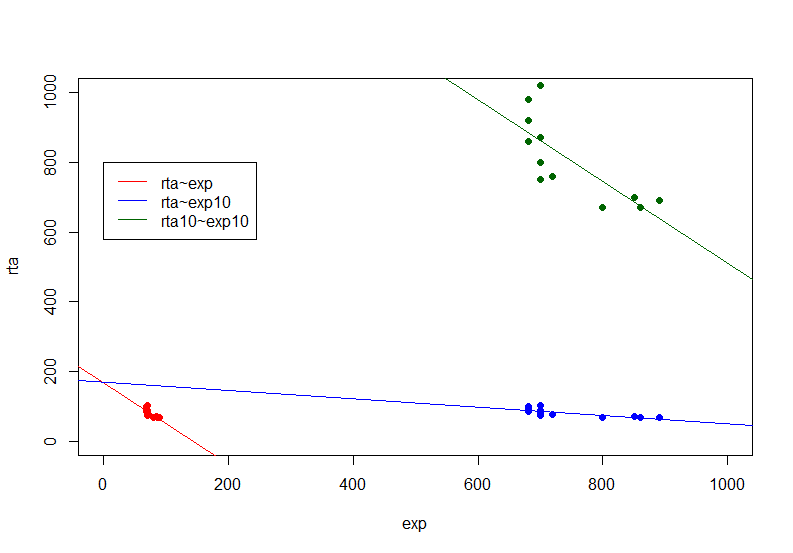
\includegraphics[width=0.8\textwidth]{5_1.png}
\caption{\label{fig:f51}Líneas de regresión.}
\end{figure}
\begin{figure}
\centering
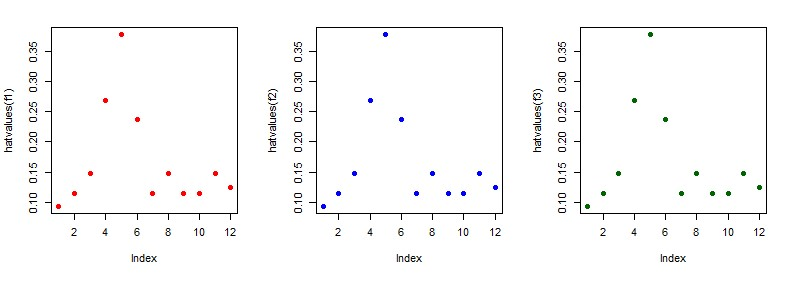
\includegraphics[width=1\textwidth]{5_2.jpg}
\caption{\label{fig:f52}Coeficientes $h_{ii}$.}
\end{figure}

Los coeficientes de cada ajuste se encuentran en la tabla~\ref{tab:51}, y en la figura~\ref{fig:f51} podemos ver los datos y las rectas de regresión. Los $h_{ii}$ correspondientes se encuentran en la tabla~\ref{tab:52} y la figura~\ref{fig:f52}. \par

Procedemos como en el ejercicio anterior, sabemos que para el ajuste sin modificaciones los coeficientes de la recta son: 
\[ \hat{\beta}_1 = \frac{\sum_{i=1}^n(x_i - \bar{x})(y_i - \bar{y})}{\sum_{i=1}^n(x_{i} - \bar{x})^2} \]
\[ \hat{\beta}_0 = \bar{y} - \hat{\beta}_1\bar{x}\]
Donde $\hat{\beta}_1$ es la pendiente y $\hat{\beta}_0$ la ordenada en el origen.\par
Al realizar la primera modificación, multiplicamos por 10 la variable $exp$, obteniendo los nuevos valores de x y su media ($exp10$): 
\[ x_{i\_exp10} = 10x_{i} \]
\[\bar{x}_{exp10} = \frac{1}{n}\sum_{i=1}^n(x_{i\_exp10}) = \frac{1}{n}\sum_{i=1}^n(10x_{i}) = 10\frac{1}{n}\sum_{i=1}^n(x_{i}) = 10\bar{x}\]
Podemos calcular los coeficientes de la recta usando $exp10$, sustituyendo los nuevos valores en la fórmula y simplificando: 
\[ \hat{\beta}_{1exp10} = \frac{\sum_{i=1}^n(x_{i\_exp10} - \bar{x}_{exp10})(y_i - \bar{y})}{\sum_{i=1}^n(x_{i\_exp10} - \bar{x}_{exp10})^2} = \frac{\sum_{i=1}^n(10x_{i} - 10\bar{x})(y_i - \bar{y})}{\sum_{i=1}^n(10x_{i} - 10\bar{x})^2} =  \]
\[ = \frac{10\sum_{i=1}^n(x_{i} - \bar{x})(y_i - \bar{y})}{100\sum_{i=1}^n(x_{i} - \bar{x})^2} = \frac{\sum_{i=1}^n(x_{i} - \bar{x})(y_i - \bar{y})}{10\sum_{i=1}^n(x_{i} - \bar{x})^2} = \frac{1}{10}\hat{\beta}_{1}  \]
\[ \hat{\beta}_{0exp10} = \bar{y} - \hat{\beta}_{1exp10}\bar{x}_{exp10} = \bar{y} - \frac{1}{10}\hat{\beta}_{1} * 10\bar{x} = \bar{y} - \hat{\beta}_{1}\bar{x} = \hat{\beta}_{0}\]
Vemos que el valor de la pendiente se ha reducido en un factor de 10, como habíamos encontrado empíricamente. Por otro lado el valor de la ordenada en el origen se mantiene constante, como nos indica la fórmula y observamos en los resultados experimentales. \par
En el segundo punto multiplicamos por 10 los valores de $rta$ que es la variable respuesta $y$, obteniendo los nuevos valores para la variable $rta10$:
\[ y_{i\_rta10} = 10y_{i}\]
\[\bar{y}_{rta10} = 10\bar{y}\]
Calculamos los coeficientes de manera similar a como hemos hecho antes:
\[ \hat{\beta}_{1exp10rta10} = \frac{\sum_{i=1}^n(x_{i\_exp10} - \bar{x}_{exp10})(y_{i\_rta10} - \bar{y}_{rta10})}{\sum_{i=1}^n(x_{i\_exp10} - \bar{x}_{exp10})^2} = \frac{\sum_{i=1}^n(10x_{i} - 10\bar{x})(10y_i - 10\bar{y})}{\sum_{i=1}^n(10x_{i} - 10\bar{x})^2} =  \]
\[ = \frac{100\sum_{i=1}^n(x_{i} - \bar{x})(y_i - \bar{y})}{100\sum_{i=1}^n(x_{i} - \bar{x})^2} = \frac{\sum_{i=1}^n(x_{i} - \bar{x})(y_i - \bar{y})}{\sum_{i=1}^n(x_{i} - \bar{x})^2} = \hat{\beta}_{1}  \]
\[ \hat{\beta}_{0exp10rta10} = \bar{y}_{rta10} - \hat{\beta}_{1exp10}\bar{x}_{exp10} = 10\bar{y} - \hat{\beta}_{1} * 10\bar{x} = 10(\bar{y} - \hat{\beta}_{1}\bar{x}) = 10\hat{\beta}_{0}\]
En esta regresión lineal obtenemos una pendiente igual a la pendiente de la recta original (sin modificaciones), y la ordenada en el origen queda multiplicada por 10.\par
Observamos que multiplicar por 10 los valores de la variable explicativa mantiene la ordenada en el origen pero divide entre 10 el valor de la pendiente. Observando la figura~\ref{fig:f51} vemos que el efecto de multiplicar por 10 (datos azules) dispersa los valores en el eje x. Al estar los valores más separados la pendiente se suaviza. Más tarde, al multiplicar por 10 la variable respuesta recuperamos el valor de la pendiente, y el valor de la ordenada en el origen se multiplica por 10 con respecto a los datos originales. En esta situación hemos multiplicado ambos datos por 10, por tanto las distancias relativas entre los puntos se mantiene, solo que con valores 10 veces mayores. En consecuencia la recta que ajusta los datos tiene la misma pendiente, pero el valor de la ordenada en el origen queda multiplicado por 10.\par
Con respecto a los valores de $h_{ii}$ vemos que son iguales para los tres ajustes. Esto se puede explicar mediante la fórmula que calcula los valores $h_{ii}$ para una regresión lineal simple:
\[ h_i = \frac{1}{n} + \frac{(x_i - \bar{x})^2}{\sum_{i'=1}^n(x_{i'} - \bar{x})^2}       \]
Al sustituir los valores de $exp10$ obtenemos: 
\[ h_{iexp10} = \frac{1}{n} + \frac{(x_{i\_exp10} - \bar{x}_{exp10})^2}{\sum_{i'=1}^n(x_{i'\_exp10} - \bar{x}_{exp10})^2} = \frac{1}{n} + \frac{(10x_i - 10\bar{x})^2}{\sum_{i'=1}^n(10x_{i'} - 10\bar{x})^2} = \frac{1}{n} + \frac{10(x_i - \bar{x})^2}{10\sum_{i'=1}^n(x_{i'} - \bar{x})^2} = h_{i}      \]
Vemos que se obtienen los mismos valores, explicando que $h_{i} = h_{iexp10}$. Por otro lado, vemos que en la fórmula no interviene la variable respuesta ($y$), por tanto al multiplicar por 10 la variable $rta$ no afecta a los valores de $h_{iexp10rta10}$, explicando que en el último ajuste se obtenga los mismos valores también.

\section{Ejercicio 6}

\textbf{Enunciado:}\par
Se ha realizado un estudio para ver si el peso en kg (\verb|rta|) de unos deportistas depende de su
cintura en cm (\verb|exp1|), del número de km de entrenamiento (\verb|exp2|) y del tipo de entrenamiento (\verb|exp3|=1: Body building, \verb|exp3|=2: Fitness). Han participado en el estudio 26 individuos. Los datos experimentales están en el fichero $c\_ccd.txt$ alojado en el curso virtual. Se ha decidido crear
las variables centradas \verb|exp1c| y \verb|exp2c| a partir de sus correspondientes \verb|exp1| y \verb|exp2|.\par
Se pide:
\begin{itemize}
    \item Interpretar los resultados del modelo de regresión lineal con todas las variables explicativas \verb|exp1c|, \verb|exp2c| y \verb|exp3|.
    \item Repetir el análisis quitando las variables no significativas. ¿Qué sucede?
    \item Crear una variable interacción entre \verb|exp1c| y \verb|exp3| e incorporarla al modelo anterior. ¿Qué ocurre?
    \item Elegir de los tres modelos anteriores el mejor. ¿Se cumplen las condiciones de aplicabilidad de la regresión lineal?
    \item Elaborar otro enunciado para estos datos.
\end{itemize}

\textbf{Solución:}\par
Código utilizado para calcular los modelos de regresión lineal:\par
\begin{lstlisting}[language=R]
rm(list=ls())
data = read.table('c_ccd.txt', header = T)
attach(data)
library (car)

exp1c = exp1 - mean(exp1) # Centrado de exp1
exp2c = exp2 - mean(exp2) # Centrado de exp2
exp3d1 = 1*(exp3 == 1) # Variable dummy exp3

f1 =lm(rta~exp1c+exp2c+exp3d1) # Regresion todas las variables
summary(f1)

f2 =lm(rta~exp1c+exp3d1) # Regresion variables significativas
summary(f2)

f3 =lm(rta~exp1c*exp3d1) # Regresion con variable de interacción
summary(f3)

detach(data)
\end{lstlisting}
El preprocesado ha consistido en centrar las variables $exp1$ y $exp2$ restando sus medias. También se ha creado una variable dummy para $exp3$, dando valor 1 cuando el entrenamiento es Body building y valor 0 cuando es fitness. Esta variable categórica al estar clasificada como 1 y 2 podría transmitir una información errónea de que la categoría 2 es más o mayor o mejor que la categoría 1, al crear la variable dummy evitamos esas falsas asociaciones y la información pasa a estar codificada de forma booleana. Como solo hay dos categorías solo necesitamos codificar una de ellas. \par
Los resultados de la regresión lineal usando todas las variables fueron los siguientes: \par
\begin{lstlisting}[language=R]
> summary(f1)

Call:
lm(formula = rta ~ exp1c + exp2c + exp3d1)

Residuals:
    Min      1Q  Median      3Q     Max 
-1.7642 -0.5996  0.1003  0.4577  1.4069 

Coefficients:
            Estimate Std. Error t value Pr(>|t|)    
(Intercept) 66.68365    0.21707  307.19  < 2e-16 ***
exp1c        0.60220    0.04326   13.92 2.18e-12 ***
exp2c        0.01173    0.02346    0.50    0.622    
exp3d1       4.16043    0.32004   13.00 8.43e-12 ***
---
Signif. codes:  0 ‘***’ 0.001 ‘**’ 0.01 ‘*’ 0.05 ‘.’ 0.1 ‘ ’ 1

Residual standard error: 0.8111 on 22 degrees of freedom
Multiple R-squared:  0.9469,	Adjusted R-squared:  0.9397 
F-statistic: 130.8 on 3 and 22 DF,  p-value: 3.551e-14
\end{lstlisting}
Vemos que para la primera variable ($exp1c$) obtenemos un coeficiente de alrededor 0.60 kg y un p-valor < 0.0001. El p-valor tan bajo nos indica que el coeficiente es significativo. Podemos concluir que por cada incremento de 1 centímetro de cintura se produce un aumento de 0.60 kg en el peso.\par
Para la segunda variable ($exp1c$) obtenemos un p-valor de 0.622, el cual nos indica que el coeficiente de esta variable (0.012 kg) no es significativamente distinto de cero. No podemos concluir que los km de entrenamiento influyan en los kg de peso. \par
Para la variable $exp3d1$ tenemos de nuevo un p-valor bajo (< 0.0001) indicándonos que el coeficiente de esta variable es significativo para el ajuste. Este coeficiente es de 4.16 kg, indicando que un atleta con un tipo de entrenamiento body building tienen aproximadamente 4.16 kg más de peso comparado con un atleta que haga fitness.\par
Por último vemos que la ordenada en el origen también es un valor relevante ya que tiene un p-valor pequeño (< 0.0001). Este coeficiente es de 66.68 kg, que como hemos centrado las variables $exp1$ y $exp2$, este valor estará cerca de la media de los pesos de los atletas (como vimos en el segundo punto del ejercicio 4).\par
Los resultados de la regresión lineal quitando la variable no significativa ($exp2c$) son: \par
\begin{lstlisting}[language=R]
> summary(f2)

Call:
lm(formula = rta ~ exp1c + exp3d1)

Residuals:
     Min       1Q   Median       3Q      Max 
-1.83742 -0.57356  0.05238  0.44248  1.29768 

Coefficients:
            Estimate Std. Error t value Pr(>|t|)    
(Intercept) 66.68204    0.21348  312.35  < 2e-16 ***
exp1c        0.60196    0.04254   14.15 7.72e-13 ***
exp3d1       4.16392    0.31471   13.23 3.07e-12 ***
---
Signif. codes:  0 ‘***’ 0.001 ‘**’ 0.01 ‘*’ 0.05 ‘.’ 0.1 ‘ ’ 1

Residual standard error: 0.7977 on 23 degrees of freedom
Multiple R-squared:  0.9463,	Adjusted R-squared:  0.9417 
F-statistic: 202.7 on 2 and 23 DF,  p-value: 2.469e-15
\end{lstlisting}
Vemos que los tres coeficientes son muy significativos con un p-valor por debajo de 0.0001. Además los valores de los tres coeficientes son prácticamente igual a los del modelo anterior con diferencias del orden de 0.001.\par
En el último modelo se pedía incluir una variable de interacción entre $exp1c$ y $exp3$:
\begin{lstlisting}[language=R]
> summary(f3)

Call:
lm(formula = rta ~ exp1c * exp3d1)

Residuals:
     Min       1Q   Median       3Q      Max 
-1.84713 -0.51997  0.07501  0.41430  1.33173 

Coefficients:
             Estimate Std. Error t value Pr(>|t|)    
(Intercept)  66.68015    0.21788 306.040  < 2e-16 ***
exp1c         0.59457    0.04942  12.030 3.79e-11 ***
exp3d1        4.15839    0.32156  12.932 9.33e-12 ***
exp1c:exp3d1  0.03230    0.10333   0.313    0.758    
---
Signif. codes:  0 ‘***’ 0.001 ‘**’ 0.01 ‘*’ 0.05 ‘.’ 0.1 ‘ ’ 1

Residual standard error: 0.8139 on 22 degrees of freedom
Multiple R-squared:  0.9466,	Adjusted R-squared:  0.9393 
F-statistic: 129.9 on 3 and 22 DF,  p-value: 3.829e-14
\end{lstlisting}
En este modelo descubrimos que la variable de interacción presenta un p-valor de 0.758, indicando que esta no es significativamente diferente de cero y no es relevante en el ajuste. Por otro lado, las variables $exp1c$ y $exp3$ siguen siendo relevantes, con p-valores bajos, y con valores para los coeficientes muy parecidos a los dos modelos anteriores.\par
Este resultado parece indicar que las dos variables $exp1c$ y $exp3$ afectan de manera independiente a la variable respuesta. El incremente en peso debido a $exp1c$ es independiente del tipo de entrenamiento, indicando que no hay sinergia entre las dos variables.\par
Entre los tres modelos se considera que el más adecuado es el segundo. En el segundo modelo todas las variables son significativas y es el modelo que menos variables tiene, lo cual lo hace más simple y menos dado al overfitting. También vemos que para el segundo modelo tenemos los valores más altos de F-statistic (un valor de 202.7 acompañado de un p-valor muy bajo, indicando que existe dependencia entre las variables explicativas y la respuesta) y Adjusted R-squared (con un valor de 0.9417, este indicador penaliza el uso de muchas variables explicativas si están no aportan nueva información. Es mejor usar este indicador para comparar modelos que R-squared, ya que R-squared siempre aumenta al incrementar el número de variables). Otro indicador importante para comparar los modelos es el RSE, disminuye cuando el ajuste es mejor y tiene en cuenta el número de parámetros. Para RSE también tenemos valores muy parecidos para los tres modelos, pero para el segundo es relativamente menor. \par

Utilizando el código \verb|plot(f2)| obtenemos las gráficas de la figura~\ref{fig:f6} que nos van a servir para estudiar la aplicabilidad del segundo modelo: \par
%independencia,
\begin{itemize}

    \item Linealidad: En la gráfica de los residuos frente a los valores vemos que no hay presencia de ningún patrón, vemos que los datos siguen la línea roja y esta se mantiene cerca de cero, indicando una buena linealidad.
    También tenemos un $R^2$ alto (0.94) indicando que los datos se ajustan a un modelo lineal.
    \item Homocedasticidad: En la gráfica de los residuos frente a los valores vemos que en todo el rango los residuos se reparten entre -1 y +1 de manera homogénea, no habiendo indicaciones de que la varianza de los residuos no sea constante. La gráfica Scale-location nos ofrece más información acerca de la homocedasticidad. En esta gráfica vemos también que las distribución de los datos es homogénea en todo el intervalo y es aproximadamente una línea recta, aunque presenta una forma ligeramente cóncava. Si realizamos el test de Breusch-Pagan para obtener indicaciones más formales, obtenemos que no podemos rechazar la hipótesis nula, denotando homocedasticidad.
    \begin{lstlisting}[language=R]
    > library(lmtest)
    > bptest(f2)

	studentized Breusch-Pagan test

    data:  f2
    BP = 0.29107, df = 2, p-value = 0.8646
    \end{lstlisting}

    \item Normalidad de los residuos: El gráfico Normal Q-Q nos permite comparar la distribución de los residuos frente a la distribución normal teórica. Por lo tanto, si los residuos tienen una distribución normal se observar que siguen aproximadamente la línea recta diagonal en el gráfico Q-Q normal, en caso contrario los residuos se van a apartar de la diagonal. En nuestro caso vemos que los residuos siguen la diagonal indicando una distribución normal.
    \item Outliers: Para estudiar los outliers nos centramos en la gráfica de Residuals vs Leverage. Aquí vemos que todos los datos se encuentra entre -2 y 2 con respecto a los residuos estandarizados. Se suele considerar outliers a partir de 3 o -3, en este caso podemos concluir que no hay outliers importantes.
    \item High Leverage Points: Podemos estudiar los puntos de alto leverage con la gráfica Residuals vs Leverage. La media de los leverages siempre está cerca de $(p+1)/n$ en nuestro caso: $(2+1)/26 = 0.12$ Podemos considerar puntos de altos leverage aquellos que excedan varias veces este valor. En nuestro caso el dato 18 es un candidato a Leverage Points ya que excede casi en 4 veces la media. Sin embargo, este punto no llega a estar fuera de la distancia de Cook de 0.5, indicando que eliminar este punto en principio no va a influir mucho en el modelo así que podemos considerar mantenerlo.
    \item Multicolinealidad: Para estudiar la multicolinealidad se calcula el factor variance inflation (VIF). Valores cercanos a 1 indican que no hay multicolinealidad, cuando exceden entre 5 y 10 indica que hay un problema muy grave de colinealidad. En este caso se obtienen unos valores muy cercanos a 1 indicando que no hay colinealidad.
\begin{lstlisting}[language=R]
> vif(f2)
   exp1c   exp3d1 
1.005607 1.005607 
\end{lstlisting}

\end{itemize}

\begin{figure}
\centering
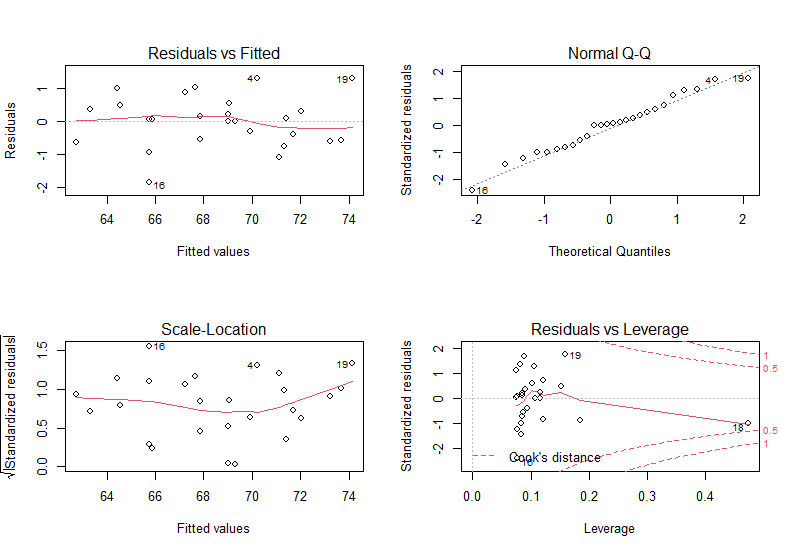
\includegraphics[width=1\textwidth]{ej6.png}
\caption{\label{fig:f6}Estudio de la aplicabilidad.}
\end{figure}
Tras estudiar los diferentes parámetros de aplicabilidad, podemos concluir que el modelo 2 es apto y cumple con los criterios de aplicabilidad. \par
Para el último apartado propongo el siguiente enunciado:\par
Se ha realizado una investigación para estudiar el número de huevos al día medio que puede producir un corral, se tienen datos de diferentes granjas (cada granja es una fila). El número de huevos medio por corral que se recogen al día en cada granja es la variable respuesta (\verb|rta|). Tenemos los siguientes datos sobre los corrales, \verb|exp1| es el número medio de gallinas por corral en cada granja, \verb|exp2| indica la calidad del alimento en una escala de 0 a 100, siendo 100 una alta calidad y 0 baja calidad. Por último tenemos \verb|exp3| que codifica con 1 si las gallinas escuchan música clásica y 2 si escuchan ruido de autopista.\par
Se pide:\par
\begin{itemize}
\item Normalizar las variables explicativas y codificar la variable categórica si es necesario.
\item Interpretar los resultados del modelo de regresión lineal con todas las variables explicativas.
\item Normalizar la variable respuesta e interpretar el nuevo modelo de regresión lineal.
\item ¿Tiene sentido la interpretación lineal del modelo cuando el número de gallinas es bajo? Por ejemplo, cuando el número de gallinas medio es 0.
\item Crear la variable $exp1^2$ y $exp2^2$ y estudiar el modelo de regresión lineal con todas las variables.
\item Seleccionar el mejor modelo e identificar si se podría mejorar eliminando alguna variable.
\item Estudiar las condiciones de aplicabilidad de la regresión lineal para el mejor modelo.
\end{itemize}



\end{document}